\label{gp_regression}
Consider the regression problem. We have a dataset $\{(x_i, f_i) | i = 1, \ldots, n\}$, which is considered to be generated from an unknown Gaussian process $f \sim \GP(m(\cdot), k(\cdot, \cdot))$, let $x \in \R^d$.  We will denote the matrix comprised of points $x_1, \ldots, x_n$ by $X \in \R^{n \times d}$ and the vector of corresponding target values $f_1, ..., f_n$ by $f \in \R^n$. We want to predict the values $f_* \in \R^l$ of the unknown process at a set of other $l$ points $X_* \in \R^{l \times d}$.

We will also consider the case, when we can't directly observe the values $f$ of the process at points $X$. Instead, we will use their noisy versions $y$, which are distributed as
$$y \sim \N(f, \sigma_n^2 I),$$
for some noise variance $\sigma_n \in \R$. The graphical model for this setting is provided in fig. \ref{gp_graphical_model}.

We will use the following notaion. We will denote the matrix, comprised of pairwise values, of covariance functions on two sets of points $A = (a_1, \ldots, a_n)^T \in \R^{n \times d}$ and $B = (b_1, \ldots, b_m)^T \in \R^{m \times d}$ by
$$K(A, B) = 
\left (\begin{array}{cccc} 
	k(a_1, b_1) & k(a_1, b_2) & \ldots & k(a_1, b_m) \\
	k(a_2, b_1) & k(a_2, b_2) & \ldots & k(a_2, b_m) \\
	\ldots & \ldots & \ldots & \ldots \\
	k(a_n, b_1) & k(a_n, b_2) & \ldots & k(a_n, b_m) \\
\end{array} \right) \in \R^{n \times m}.
$$

Then, the joint distribution of $f$ and $f_*$ is given by
$$
\left [ \begin{array}{c} f\\ f_* \end{array} \right ]
\sim
\N \left ( 0, \left [\begin{array}{cc} K(X, X) & K(X, X_*)\\ K(X_*, X) & K(X_*, X_*) \end{array} \right] \right ).
$$

\begin{figure}[!h]
	\centering
	\scalebox{0.9}{
		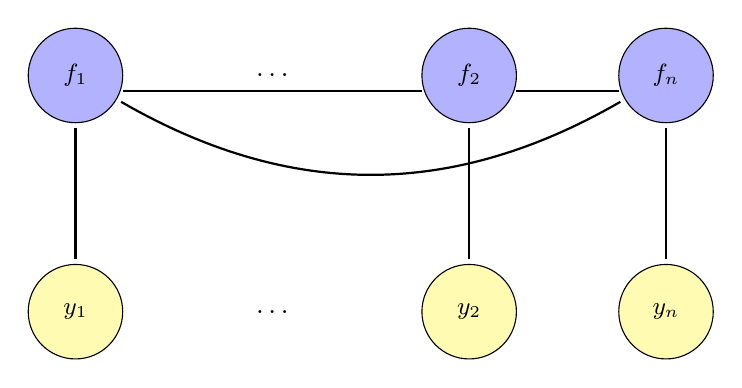
\begin{tikzpicture}
	\tikzstyle{x_i} = [circle, draw, fill=green!50, minimum size=1.2cm, text width=0.8cm, align=center, font=\large]
	\tikzstyle{f_i} = [circle, draw, fill=blue!30, minimum size=1.2cm, inner sep=2pt, outer sep=2pt, font=\small, align=center]
	\tikzstyle{y_i} = [circle, draw, fill=yellow!30, minimum size=1.2cm, inner sep=2pt, outer sep=2pt, font=\small, align=center]
	\tikzstyle{edge_label} = [font=\small, label={[label distance = -4pt]90:$\text$}]
	\tikzstyle{edge} = [thick, >=stealth]
	\tikzstyle{biedge} = [thick, >=stealth]
	\def\step{-3}
	\def\layerpos{3}

	\foreach \name/\x in {f_1/-2.5, f_2/2.5, f_n/5} 
	  	\node[f_i] (\name) at (\x, \layerpos) {$\name$};

	\draw[biedge] (f_1)++(0.6,-0.2) -- ++(3.8,0); %(f_2);
	\draw[biedge] (f_2)++(0.6,-0.2) -- +(1.3,0);% ++ (f_n);
	\draw [biedge] (f_1) to [out=-30,in=-150] (f_n);
	\node (other^2) at (0, \layerpos) {$\ldots$};

	%observables
	\pgfmathsetmacro{\layerpos}{\layerpos + \step}

	\foreach \name/\x in {y_1/-2.5, y_2/2.5, y_n/5} 
	  	\node[y_i] (\name) at (\x, \layerpos) {$\name$};

	\node (other^3) at (0, \layerpos) {$\ldots$};
	\foreach \from/\to in {f_1/y_1, f_2/y_2, f_n/y_n}
		\draw[edge] (\from) -- (\to);
\end{tikzpicture}
	}
	\caption{The graphical model for Gaussian process regression and classification}
	\label{gp_graphical_model}
\end{figure}

As $y$ is obtained by adding a normally distributed noise to $f$, the joint distribution

$$
\left [ \begin{array}{c} y\\ f_* \end{array} \right ]
\sim
\N \left ( 0, \left [\begin{array}{cc} K(X, X) + \sigma_n^2 I & K(X, X_*)\\ K(X_*, X) & K(X_*, X_*) \end{array} \right] \right ).
$$

Conditioning this distribution, we obtain the predictive


$$f_* | X_*, X, f \sim \N( \hat m, \hat K ),$$
where 
$$\E [f_* | f ] = \hat m = K(X_*, X) K(X, X)^{-1} f,$$
$$\cov(f_* | f ) = \hat K = K(X_*, X_*) - K(X_*, X)K(X, X)^{-1}K(X, X_*).$$

Thus, the complexity of obtaining the predictive distribution, is determined by the complexity of inverting the $n$ by $n$ matrix $K(X, X)$ and thus scales as $\bigO(n^3)$.

\begin{figure}[!h]
	\centering
	\subfloat{
		\scalebox{0.7}{
			\input{../../Code/Experiments/pictures/1dgp-regression.pgf}
		}
	}
	\subfloat{
		\scalebox{0.7}{
    		\input{../../Code/Experiments/pictures/2dgp-regression.pgf}
		}
	}
	\caption{One and two-dimensional Gaussian processes, reconstructed from data}
	\label{brute_reg_example}
\end{figure}


In fig. \ref{brute_reg_example} you can see the examples of one and two-dimensional Gaussian processes, reconstructed from the data. The data points are shown by black `$+$' signs. 

For more detailed description of Gaussian process regression see \cite{GPinML}.